\section{评估}
\label{sec:evaluation}

\subsection{实验设置}

\parab{测试平台设置。}
测试平台由 8 台服务器组成，每台服务器配备 4 块 NVIDIA GeForce RTX 3090 GPU、40 个 CPU 核（Intel(R) Xeon(R) Gold 5218R CPU @ 2.10GHz）、128GB 内存以及两张 ConnectX-5 100Gbps NIC。服务器通过 NVIDIA SN2700 以太网交换机互连。单机内部 GPU 通过 PCIe Gen 3.0 通信。所有服务器运行 Ubuntu 22.04、CUDA 12.8、PyTorch 2.8.0 和 NCCL 2.28。我们配置了一个由 16 块 GPU 组成的 prefill 集群，并单独配置 decode worker。为简化分析，我们将 decode 输出长度限制为 1 个 token，因为这不会影响 TTFT。

\parab{仿真设置。}
我们的模拟器构建在 Vidur~\cite{agrawal2024vidur} 与流级模拟器 flowsim~\cite{FlowSim2024} 之上。我们扩展了 Vidur，使其支持带专家并行和序列并行的 Mixtral 模型，以及带 KV-cache 复用的 PD 解耦。仿真流程首先通过 Vidur profiler 离线剖析算子时延；运行时，我们采用统一的事件驱动机制：Vidur 负责模拟 LLM 服务行为并生成计算与通信任务，而 flowsim 负责解析通信任务并触发底层网络事件。关键在于，计算事件与网络事件都在同一个事件队列中处理，以保证正确性。默认情况下，我们模拟一个 256 台服务器的集群，prefill 与 decode worker 比例为 1:1，并由一个类似 Dynamo~\cite{NVIDIA_Dynamo} 的 KV-cache 感知调度器统一管理。每台服务器包含 8 块通过 NVSwitch（900 GB/s）互连的 GPU 和 8 张 NIC，整个系统采用 1:1 fat-tree 网络，链路带宽为 200Gbps。时延剖面基于 NVIDIA A100 GPU 标定。

\parab{指标。}
我们主要评估首 Token 时间（TTFT）及其服务级目标（SLO）达成率。遵循~\cite{patke2024queue,hongsola,stojkovic2025dynamollm} 的方法，默认将 SLO 阈值定义为低负载条件下 TTFT 的 $3\times$。我们也评估了一些微基准指标，例如集合通信完成时间（CCT）和请求提前量（earliness），以帮助解释性能收益来源。

\subsection{测试平台实验}
\label{sec:evaluation:testbed}

\begin{figure}[t!]
    \centering
    \begin{subfigure}[t]{0.48\linewidth}
        \centering
        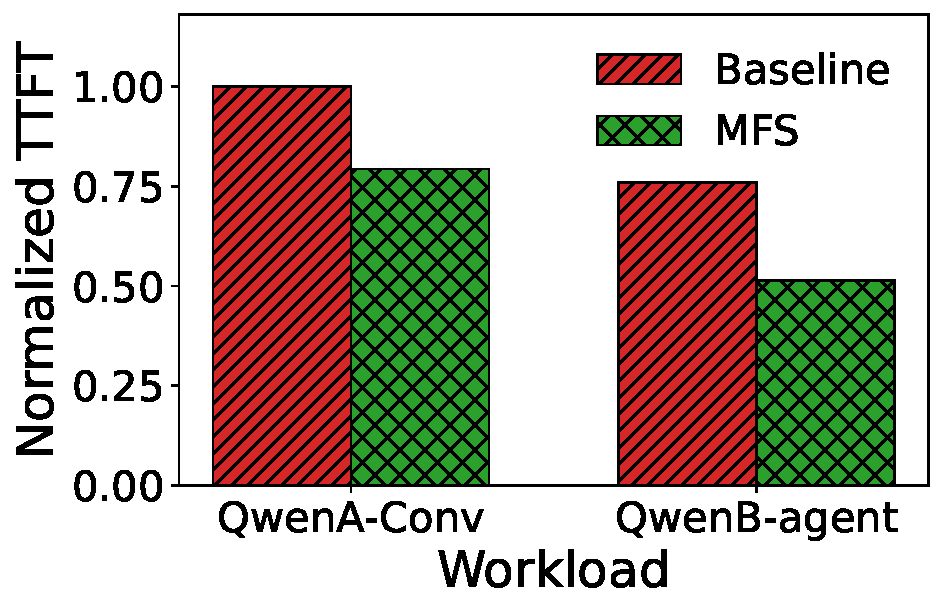
\includegraphics[width=\linewidth]{figures/evaluation/testbed/mixtral_TTFT_mfs.pdf}
        \caption{归一化 TTFT。}
        \label{fig:evaluation:testbed:ttft}
    \end{subfigure}
    \hfill
    \begin{subfigure}[t]{0.48\linewidth}
        \centering
        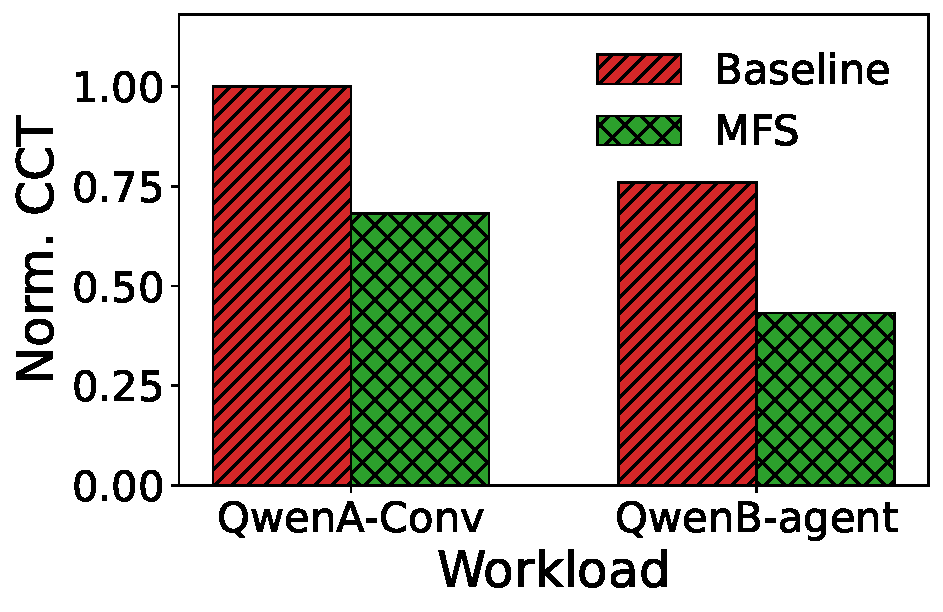
\includegraphics[width=\linewidth]{figures/evaluation/testbed/mixtral_alltoall_mfs.pdf}
        \caption{归一化 CCT。}
        \label{fig:evaluation:testbed:cct}
    \end{subfigure}
    \hfill
    \caption{【测试平台】Mixtral-8x7B}
    \label{fig:evaluation:testbed}
\end{figure}


\input{sections/fig_code/evaluation/sim_qwenA_zh}
\begin{figure*}[ht!]
    \begin{subfigure}[b]{0.24\linewidth}
        \centering
        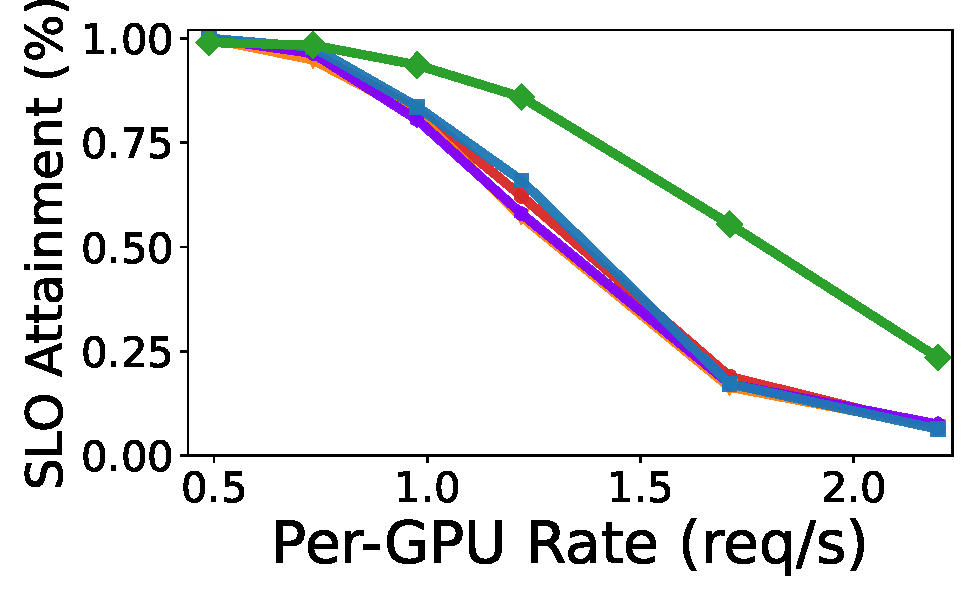
\includegraphics[width=\linewidth]{figures/evaluation/sim_qwenB/QwenB_mixtral8x22B_bw200.pdf}
        \caption{Mixtral-8x22B}
        \label{fig:evaluation:qwenB:mixtral_200}
    \end{subfigure}
    \hfill
    \begin{subfigure}[b]{0.24\linewidth}
        \centering
        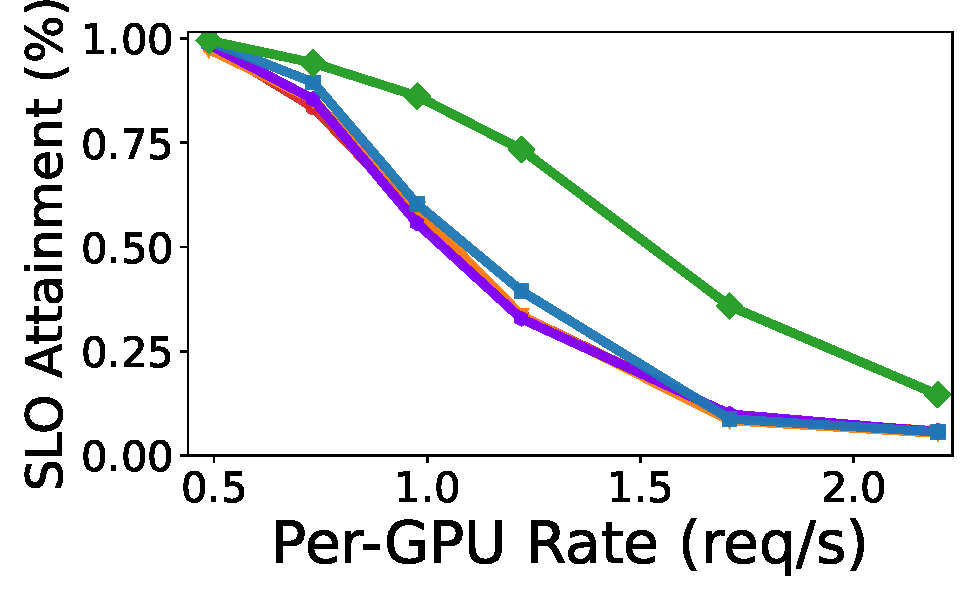
\includegraphics[width=\linewidth]{figures/evaluation/sim_qwenB/QwenB_DBRX_bw200.pdf}
        \caption{DBRX}
        \label{fig:evaluation:qwenB:DBRX}
    \end{subfigure}
    \hfill
    \begin{subfigure}[b]{0.24\linewidth}
        \centering
        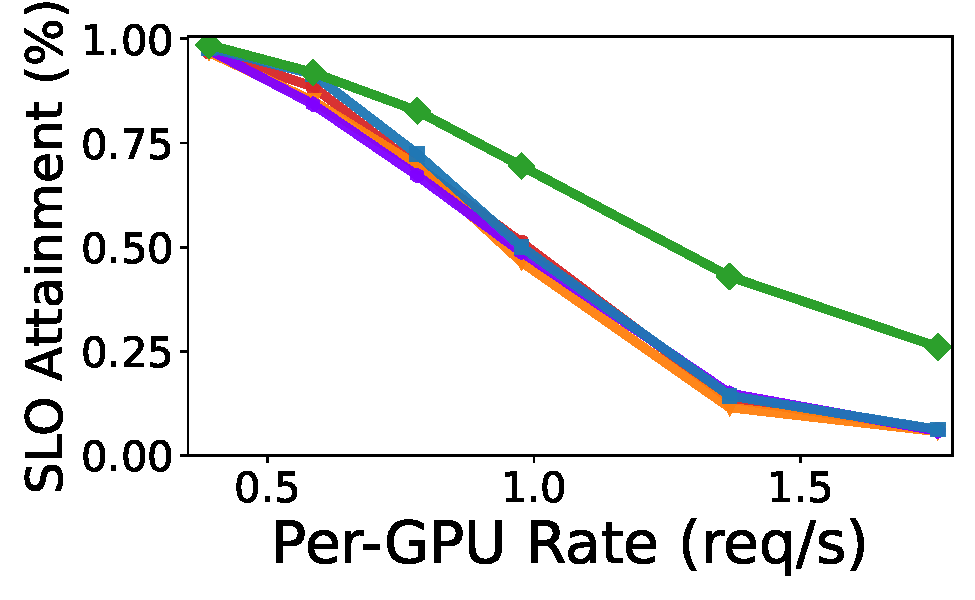
\includegraphics[width=\linewidth]{figures/evaluation/sim_qwenB/QwenB_coder_bw200.pdf}
        \caption{Qwen3-Coder}
        \label{fig:evaluation:qwenB:qwencoder_200}
    \end{subfigure}
    \hfill
    \begin{subfigure}[b]{0.24\linewidth}
        \centering
        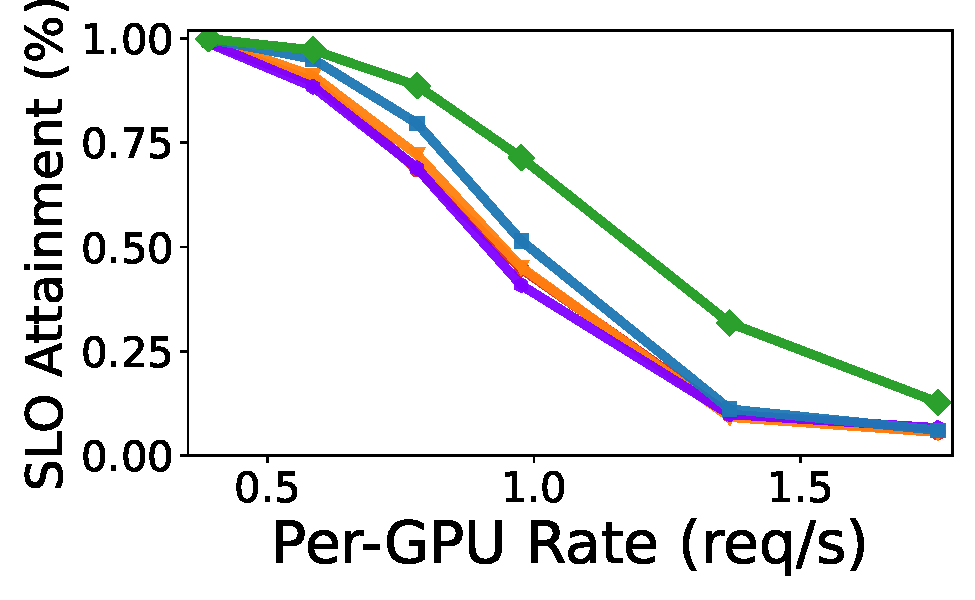
\includegraphics[width=\linewidth]{figures/evaluation/sim_qwenB/QwenB_grok2_bw200.pdf}
        \caption{Grok2}
        \label{fig:evaluation:qwenB:grok2_200}
    \end{subfigure}
    \vspace{-0.3cm}
    \caption{【仿真】智能体工作负载（QwenB）上的性能}
    \label{fig:evaluation:qwenB}
\end{figure*}


\parab{模型与工作负载。}
在测试平台实验中，我们评估 Mistral 8x7B~\cite{mixtral7b} MoE 模型（FP16，top-$k$=2），其张量并行度（TP）设置为 1，专家并行度（EP）设置为 8。工作负载方面，我们采用两条来自 Qwen 的生产轨迹~\cite{qwen_bailian_traces}。其中，QwenA-Conv 表示\textit{对话型工作负载}，平均序列长度为 2k token，prompt 复用率为 50\%；QwenB-agent 表示\textit{智能体型工作负载}，平均长度为 1k token，复用率更高，为 65\%。请求到达遵循泊松过程，我们通过调整每秒请求数（RPS）来控制系统负载。受测试平台容量限制，我们将每条轨迹的前 512 个请求作为预热阶段，并使用之后的 1024 个请求进行评估。

图~\ref{fig:evaluation:testbed} 展示了 \sys{} 在 QwenA-Conv 与 QwenB-Agent 两类工作负载上的表现。我们将 vLLM 的 batched tokens 设置为 8192，并将每 GPU 请求率设为每秒 1 个请求。\sys{} 在两种工作负载下都显著降低了 TTFT：在 QwenA-Conv 上，平均 TTFT 优化 20.7\%（1.26$\times$）；在 QwenB-Agent 上，优化 32.3\%（1.48$\times$）。TTFT 的下降主要来自于阻塞计算的集合通信更快完成。以 all-to-all 完成时间（CCT）为例，\sys{} 在 QwenA-Conv 上将阶段 2 通信缩短 31.9\%（1.47$\times$），在 QwenB-Agent 上缩短 43.1\%（1.76$\times$）。这些集合通信处于 prefill 执行的关键路径上：一旦被拖慢，就会立即阻塞 GPU 计算并抬高端到端延迟。

\subsection{大规模仿真}

在大规模仿真中，我们扩大了评估范围，以覆盖多种生产级架构与工作负载。
\begin{itemize}[leftmargin=*]
    \item 我们考察了一组主流的专家并行 MoE 模型：既包括专家规模大但数量较少的架构（如 Mixtral 8x22B~\cite{mixtral22b} 和 Grok-2~\cite{grok}，配置为 TP=4, EP=8），也包括专家更小但数量更多的模型（如 DBRX~\cite{dbrx}，配置为 TP=2, EP=16，以及 Qwen3-Coder~\cite{qwen-coder}，配置为 TP=1, EP=32）。这些模型均部署在 32-GPU 实例上，并采用混合并行策略。我们利用 Qwen 对话轨迹与智能体轨迹来代表典型交互行为。
    \item 我们还进一步评估 \sys{} 在采用序列并行（SP）的稠密模型上的有效性~\cite{ringattention}。我们评估了配置为 1M token 上下文窗口的 Llama~\cite{llama} 模型。在该设置下，模型部署于 16-GPU 实例上，采用 TP=4、SP=4。我们将其与 Mooncake 数据集~\cite{mooncake}配对，以模拟具有相似复用率（约 $\sim40\%$、$\sim65\%$）和更长上下文长度（约 $\sim15k$、$\sim9k$）的真实对话和智能体工作负载。
\end{itemize}

\parab{基线。} 我们将 \sys{} 与四类经典流调度策略进行比较：
\begin{itemize}[leftmargin=*]
    \item \textbf{Fair Sharing}：对并发流实施 max-min 公平，按等带宽分配，不考虑流大小与截止时间。
    \item \textbf{Shortest Job First（SJF）}：严格优先调度更小的流，以最小化平均流完成时间。
    \item \textbf{Earliest Deadline First（EDF）}：优先调度带显式截止时间的流。由于应用级截止时间无法直接映射为单个网络流截止时间，对带隐式截止时间的流则退化为公平共享。
    \item \textbf{Karuna~\cite{karuna}}：为带截止时间的流分配确保按时完成所需的最小带宽，而剩余流量按 SJF 调度。
\end{itemize}

\parab{端到端 TTFT SLO 达成率。} 我们在不同请求率、不同模型与工作负载下评估端到端 TTFT SLO 达成率。结果如图~\ref{fig:evaluation:qwenA}、\ref{fig:evaluation:qwenB} 和 \ref{fig:evaluation:sp} 所示，\sys{} 在所有场景中都稳定优于当前最先进的基线方案。

图~\ref{fig:evaluation:qwenA} 展示了 \sys{} 在多种 MoE 模型上的对话工作负载表现。具体来说，在高请求率下，\sys{} 在 Mixtral（图~\ref{fig:evaluation:qwenA:mixtral_200}）、Qwen Coder（图~\ref{fig:evaluation:qwenA:qwencoder_200}）和 Grok（图~\ref{fig:evaluation:qwenA:grok2_200}）上的 SLO 达成率提升为 1.4$\times$--1.8$\times$，而在 DBRX（图~\ref{fig:evaluation:qwenA:dbrx_200}）上最高达到 2.4$\times$。此外，在维持相近 SLO 达成率的前提下，\sys{} 能承受比最强基线 Karuna 高出 1.17$\times$--1.46$\times$ 的请求率。在对话工作负载中，一小部分尾部请求需要大规模 KV-cache 迁移，这会在高负载下触发从阶段 1 到阶段 3 的跨阶段争用。\sys{} 能显著优于基线，正是因为它成功协调了多阶段争用。在各基线中，Karuna 相对表现较好，因为它\emph{碰巧}会延后非紧急的阶段 3 流量，从而提供一定缓解；但由于缺乏显式的多阶段协同，它最终仍会像其他基线一样被争用拖垮。

图~\ref{fig:evaluation:qwenB} 展示了 \sys{} 在多种 MoE 模型上的智能体工作负载表现。聚焦中高负载区间，\sys{} 在 Grok-2 与 Mixtral 上实现 1.4$\times$--1.7$\times$ 更高的 SLO 达成率，在 DBRX 和 Qwen-Coder 上可达到 2.0$\times$。此外，与 Karuna 相比，\sys{} 可支持 Grok-2 高出 1.2$\times$ 的请求率，Mixtral 和 Qwen-Coder 约高出 $\sim1.3\times$，DBRX 则可达 1.4$\times$。相较于对话轨迹，智能体请求的 prompt 更短，但平均复用率更高，多个并发请求经常共享完全相同的前缀。这种模式诱发了严重的一对多发送端争用，其主要集中在阶段 1 和阶段 2，因为多个 worker 会同时争抢同一批缓存状态。\sys{} 无需精确松弛度估计，就能通过保护紧急流有效缓解这种争用。值得注意的是，在该场景下，Karuna 与其他基线之间的差距有所缩小。当争用并非主要由阶段 3 流量主导时，Karuna 会退化为使用 SJF 来调度阶段 1 和阶段 2 流（因为截止时间是隐式的）；然而，由于其不理解阶段语义，这种做法仍然会像其他基线一样，让紧迫请求暴露于 SLO 违约风险之下。

\begin{figure}[t!]
    \centering
    \begin{subfigure}[b]{0.48\linewidth}
        \centering
        
\includegraphics[width=\linewidth]{figures/evaluation/sim_mc_conv/llama3_bw200_mfs.pdf}
        \caption{对话工作负载}
        \label{fig:evaluation:sp:conv}
    \end{subfigure}
    \hfill
    \begin{subfigure}[b]{0.48\linewidth}
        \centering
        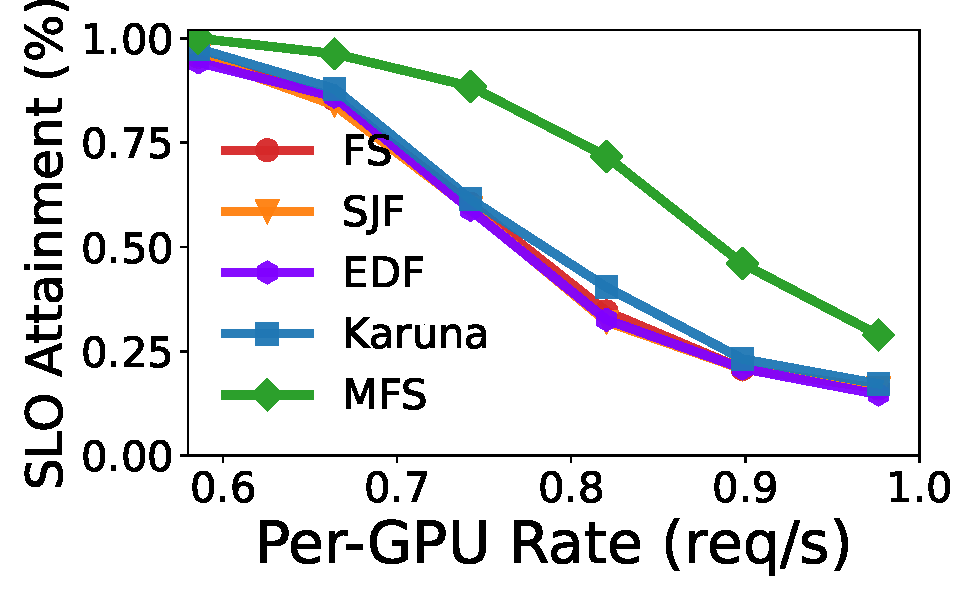
\includegraphics[width=\linewidth]{figures/evaluation/sim_mc_agent/llama3_bw200_mfs.pdf}
        \caption{智能体工作负载}
        \label{fig:evaluation:sp:agent}
    \end{subfigure}
    \hfill
    \vspace{-0.3cm}
    \caption{【仿真】Llama3-8B（Mooncake 数据集）}
    \label{fig:evaluation:sp}
\end{figure}

图~\ref{fig:evaluation:sp} 展示了 \sys{} 在采用序列并行（SP）的 Llama3-8B 模型上、两个代表性长上下文工作负载中的表现。对于 Mooncake 数据集，对话与智能体工作负载在请求模式上与 Qwen 实验相似（例如复用率、访问模式），但上下文长度显著更长。在对话工作负载中（图~\ref{fig:evaluation:sp}a），\sys{} 在负载上升时依然表现稳健，相比 Karuna 实现了 1.3$\times$--1.6$\times$ 的 SLO 达成率提升。这一优势在智能体工作负载中进一步放大（图~\ref{fig:evaluation:sp}b）：\sys{} 实现了 1.4$\times$--1.9$\times$ 的更高 SLO 达成率，并在严格 SLO 预算下支持最高 1.15$\times$ 的每 GPU 请求率提升。

\parab{性能收益拆解。} 我们进一步设计了微基准实验，以分析收益来源。正如图~\ref{fig:evaluation:qwenA:dbrx:mb} 与图~\ref{fig:evaluation:sp_mb} 所示，\sys{} 成功实现了两点：
(i) 最小化集合通信完成时间（即非重叠通信时延），从而缩短 prefill 总工期；
(ii) 调控提前量，在争用条件下优先保障真正紧急的请求。

图~\ref{fig:evaluation:qwenA:dbrx:mb} 对 \sys{} 在 DBRX 模型上实现 2.2$\times$ 更高 SLO 达成率的收益进行了拆解。
第一项收益来自 prefill 阶段执行时间的缩短。具体而言，\sys{} 将专家并行的平均 CCT 降低了 52\%（图~\ref{fig:evaluation:qwenA:dbrx:cascading}）。这一收益主要来源于我们的阶段感知策略：它优先保护会阻塞计算的流，同时延后非关键流量，以利用可用松弛度实现重叠。
因此，\sys{} 通过降低有效通信开销，显著缩短了 prefill 总工期。

\begin{figure}[t!]
    \centering
    \begin{subfigure}[t]{0.48\linewidth}
        \centering
        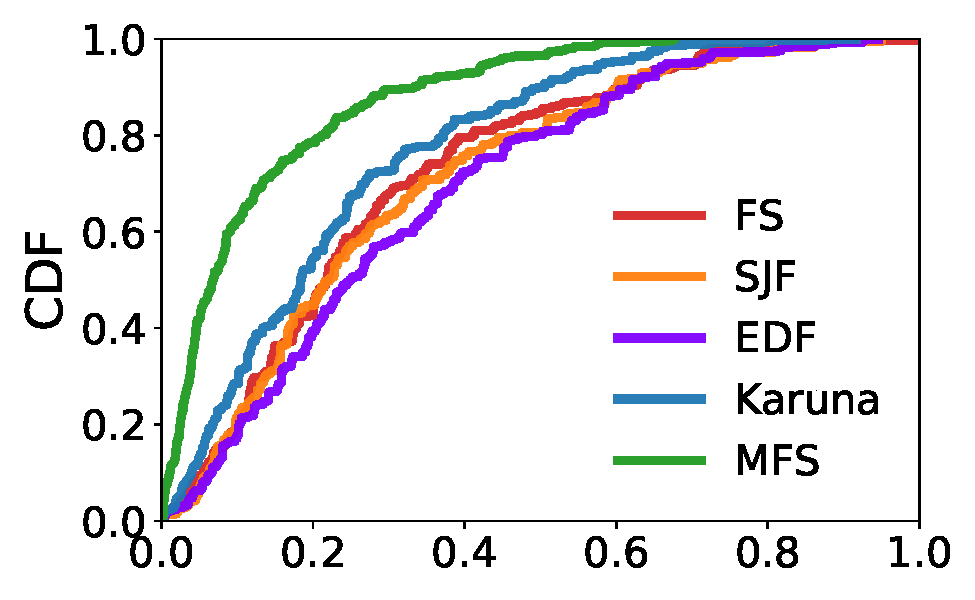
\includegraphics[width=\linewidth]{figures/evaluation/sim_qwenA/dbrx_bw200_cascading_delay_cdf_mfs.pdf}

        \caption{归一化 CCT。}
        \label{fig:evaluation:qwenA:dbrx:cascading}
    \end{subfigure}
    \hfill
    \begin{subfigure}[t]{0.48\linewidth}
        \centering
        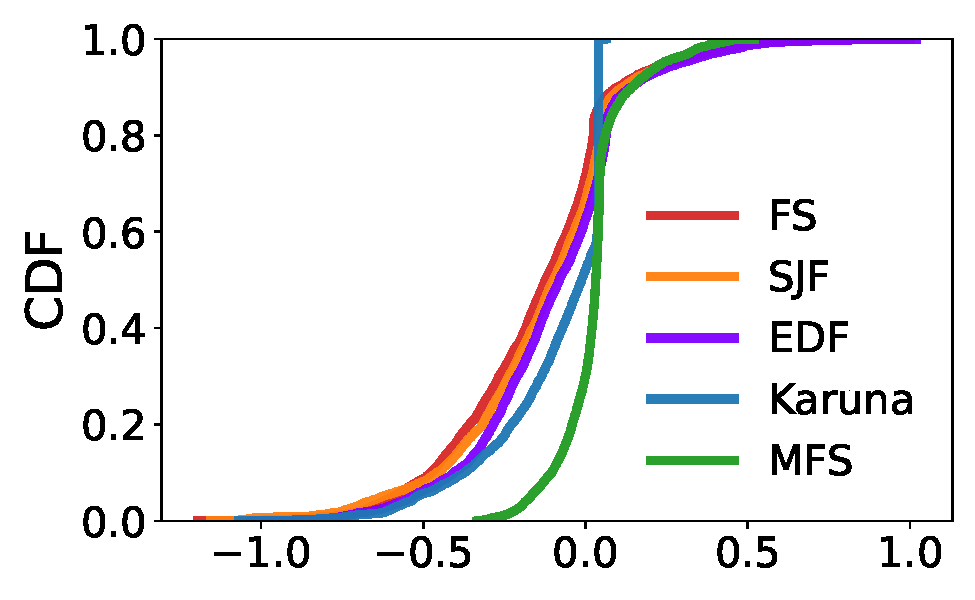
\includegraphics[width=\linewidth]{figures/evaluation/sim_qwenA/dbrx_bw200_earliness_cdf_mfs.pdf}
        \caption{归一化提前量。}
        \label{fig:evaluation:qwenA:dbrx:earliness}
    \end{subfigure}
    \hfill
    \caption{【仿真】DBRX 上的收益拆解（Qwen-A，Rate=0.7）}
    \label{fig:evaluation:qwenA:dbrx:mb}

\end{figure}

\begin{figure}[t!]
    \centering
    \begin{subfigure}[t]{0.48\linewidth}
        \centering
        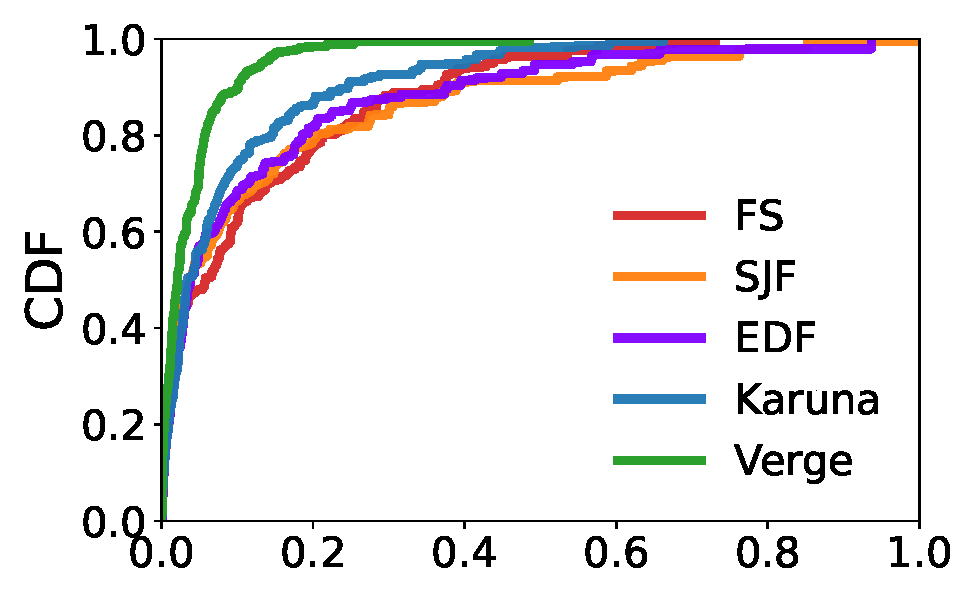
\includegraphics[width=\linewidth]{figures/evaluation/sim_mc_agent/cascading_delay_cdf.pdf}

        \caption{归一化 CCT。}
        \label{fig:evaluation:sp:cascading}
    \end{subfigure}
    \hfill
    \begin{subfigure}[t]{0.48\linewidth}
        \centering
        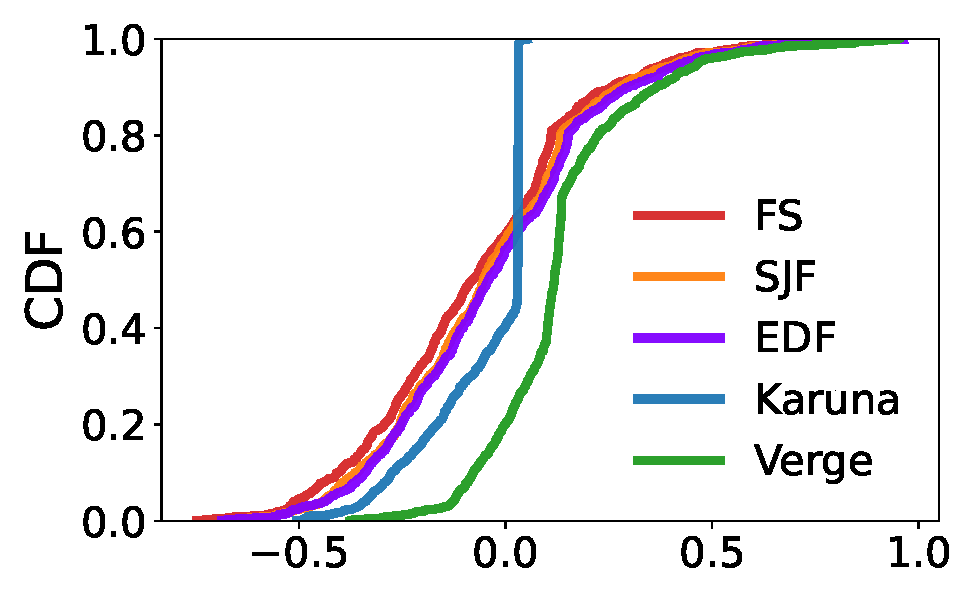
\includegraphics[width=\linewidth]{figures/evaluation/sim_mc_agent/request_earliness_cdf.pdf}

        \caption{归一化提前量}
        \label{fig:evaluation:sp:earliness}
    \end{subfigure}
    \hfill
    \caption{【仿真】Llama3 上的收益拆解（Mooncake-Conv，Rate=0.5）}
    \label{fig:evaluation:sp_mb}
    \vspace{-0.5em}
\end{figure}


除了降低时延外，\sys{} 还通过更准确地优先真正紧急的请求，进一步提升了 SLO 达成率。
我们使用请求的\emph{提前量}（earliness）来刻画这一现象：较大的正值意味着不必要的过早完成，这会阻塞更紧急的请求；负值则对应截止违约。
如图~\ref{fig:evaluation:qwenA:dbrx:earliness} 所示，Karuna 的非负提前量最小，但其代价是更高的违约风险，因为它采用近乎最小速率的保守分配方式，无法有效利用可用带宽。
相比之下，其他基线表现出更大的非负提前量，说明它们在调度流时没有有效体现紧迫性。
与 FS、SJF、EDF 相比，\sys{} 将非负部分的提前量降低了 42\%。通过把阶段 3 流量延后到\textit{恰好按时完成}，并利用基于 RED 的排序来调控早期阶段流量，\sys{} 为真正紧急的请求保留了资源。\sys{} 同时采用基于优先级的调度方式，因此在没有更高优先级流等待时，仍可充分利用可用带宽。

我们在图~\ref{fig:evaluation:sp_mb} 中观察到了相似趋势。
在这两组微基准中，\sys{} 都通过同时降低序列并行的集合通信完成时间（图~\ref{fig:evaluation:sp:cascading}）并调控争用下的提前量（图~\ref{fig:evaluation:sp:earliness}），稳定实现更高的 SLO 达成率。
这些结果表明，\sys{} 的性能收益在不同模型间具有稳健性，并不依赖某一种特定工作负载或架构。
